\documentclass[aspectratio=169, french]{ISAE-Beamer}
\usepackage{fontspec}
%\usepackage[french]{babel}
\usefonttheme[onlymath]{serif}
\usepackage{amsmath,amssymb,amsthm}
\usepackage{arydshln,mathtools}
\usepackage{bm}
\usepackage{color}
\definecolor{theme}{RGB}{0,73,114}
\usepackage{multicol}
%\usepackage[caption=false]{subfig}
\usepackage{subcaption}

\usepackage{comment}

\usepackage{graphicx}
\usepackage{diffcoeff}
\usepackage{dsfont}
\usepackage{mathrsfs}
\usepackage[most]{tcolorbox}

\usepackage{xspace}
\usepackage{appendixnumberbeamer}


\usepackage{media9}
\usepackage[backend=bibtex,style=verbose,doi=false,isbn=false,url=false,eprint=false,autocite=footnote]{biblatex}

\addtobeamertemplate{footnote}{\vspace{-6pt}\advance\hsize-0.5cm}{\vspace{6pt}}
\makeatletter
% Alternative A: footnote rule
\renewcommand*{\footnoterule}{\kern -3pt \hrule \@width 2in \kern 8.6pt}
% Alternative B: no footnote rule
% \renewcommand*{\footnoterule}{\kern 6pt}
\makeatother

\graphicspath{{./images/}}

\bibliography{biblio_pres}

% Math macros
\DeclareMathOperator*{\grad}{grad}
\DeclareMathOperator*{\Grad}{Grad}
\DeclareMathOperator*{\Div}{Div}
\renewcommand{\div}{\operatorname{div}}
\DeclareMathOperator*{\Hess}{Hess}
\DeclareMathOperator*{\curl}{curl}
\DeclareMathOperator{\Tr}{Tr}
\DeclareMathOperator{\Dom}{Dom}
\DeclareMathOperator*{\esssup}{ess\,sup}

\newcommand{\bbR}{\mathbb{R}}
\newcommand{\bbF}{\mathbb{F}}
\newcommand{\bbA}{\mathbb{A}}
\newcommand{\bbB}{\mathbb{B}}
\newcommand{\bbS}{\mathbb{S}}

\newcommand*{\norm}[1]{\ensuremath{\left\|#1\right\|}}
\newcommand{\where}{\qquad \text{where} \qquad}
\newcommand{\inner}[3][]{\ensuremath{\left\langle #2, \, #3 \right\rangle_{#1}}}
\newcommand{\bilprod}[2]{\left\langle \left\langle \, #1, #2 \, \right\rangle \right\rangle}
\newcommand{\pder}[2]{\ensuremath{\partial_{#2} #1}}
\newcommand{\dder}[2]{\ensuremath{\delta_{#2} #1}}
\newcommand{\secref}[1]{\S\ref{#1}}
\newcommand{\energy}[1]{\frac{1}{2} \int_{\Omega} \left\{ #1 \right\} \d\Omega}
\newcommand{\crmat}[1]{\ensuremath{\left[#1\right]_\times}}
\newcommand{\fenics}{\textsc{FEniCS}\xspace}
\newcommand{\firedrake}{\textsc{Firedrake}\xspace}

\DeclareMathOperator*{\argmax}{arg\,max}
\DeclareMathOperator*{\argmin}{arg\,min}

\newtheorem{proposition}{Proposition}
\newtheorem{remark}{Remark}
\newtheorem{hypothesis}{Hypothesis}
\newtheorem{assumption}{Assumption}
\newtheorem{conjecture}{Conjecture}


\def\onedot{$\mathsurround0pt\ldotp$}
\def\cddot{% two dots stacked vertically
	\mathbin{\vcenter{\baselineskip.67ex
			\hbox{\onedot}\hbox{\onedot}}%
}}

\renewcommand\bibfont{\scriptsize}


\makeatletter \renewcommand\d[1]{\ensuremath{%
		\;\mathrm{d}#1\@ifnextchar\d{\!}{}}}
\makeatother


\graphicspath{{./images/}}

\title[Projet d'intégration]{Projet d'intégration pour le poste\\ \small
\textit{Enseignant-Chercheur en Méthodes Mathématiques pour le Calcul Scientifique}}


\author[Andrea Brugnoli]{Andrea Brugnoli}

\date[11/4/22]{11 Avril 2022}

%\thanks{}



\begin{document}
	
	
	\maketitle
	
	
	\begin{frame}{Outline}
		
		\tableofcontents
		
	\end{frame}
	
	\section{Enjeux du poste}
	
	\begin{frame}{La simulation numérique au service de l'ingénierie}
		Ce poste s'inscris dans la thématique Science Computationnelle et Ingénierie\footcite{ulrich2018cse}.
		
		\begin{columns}
			\begin{column}{.45\textwidth}
			\begin{figure}
				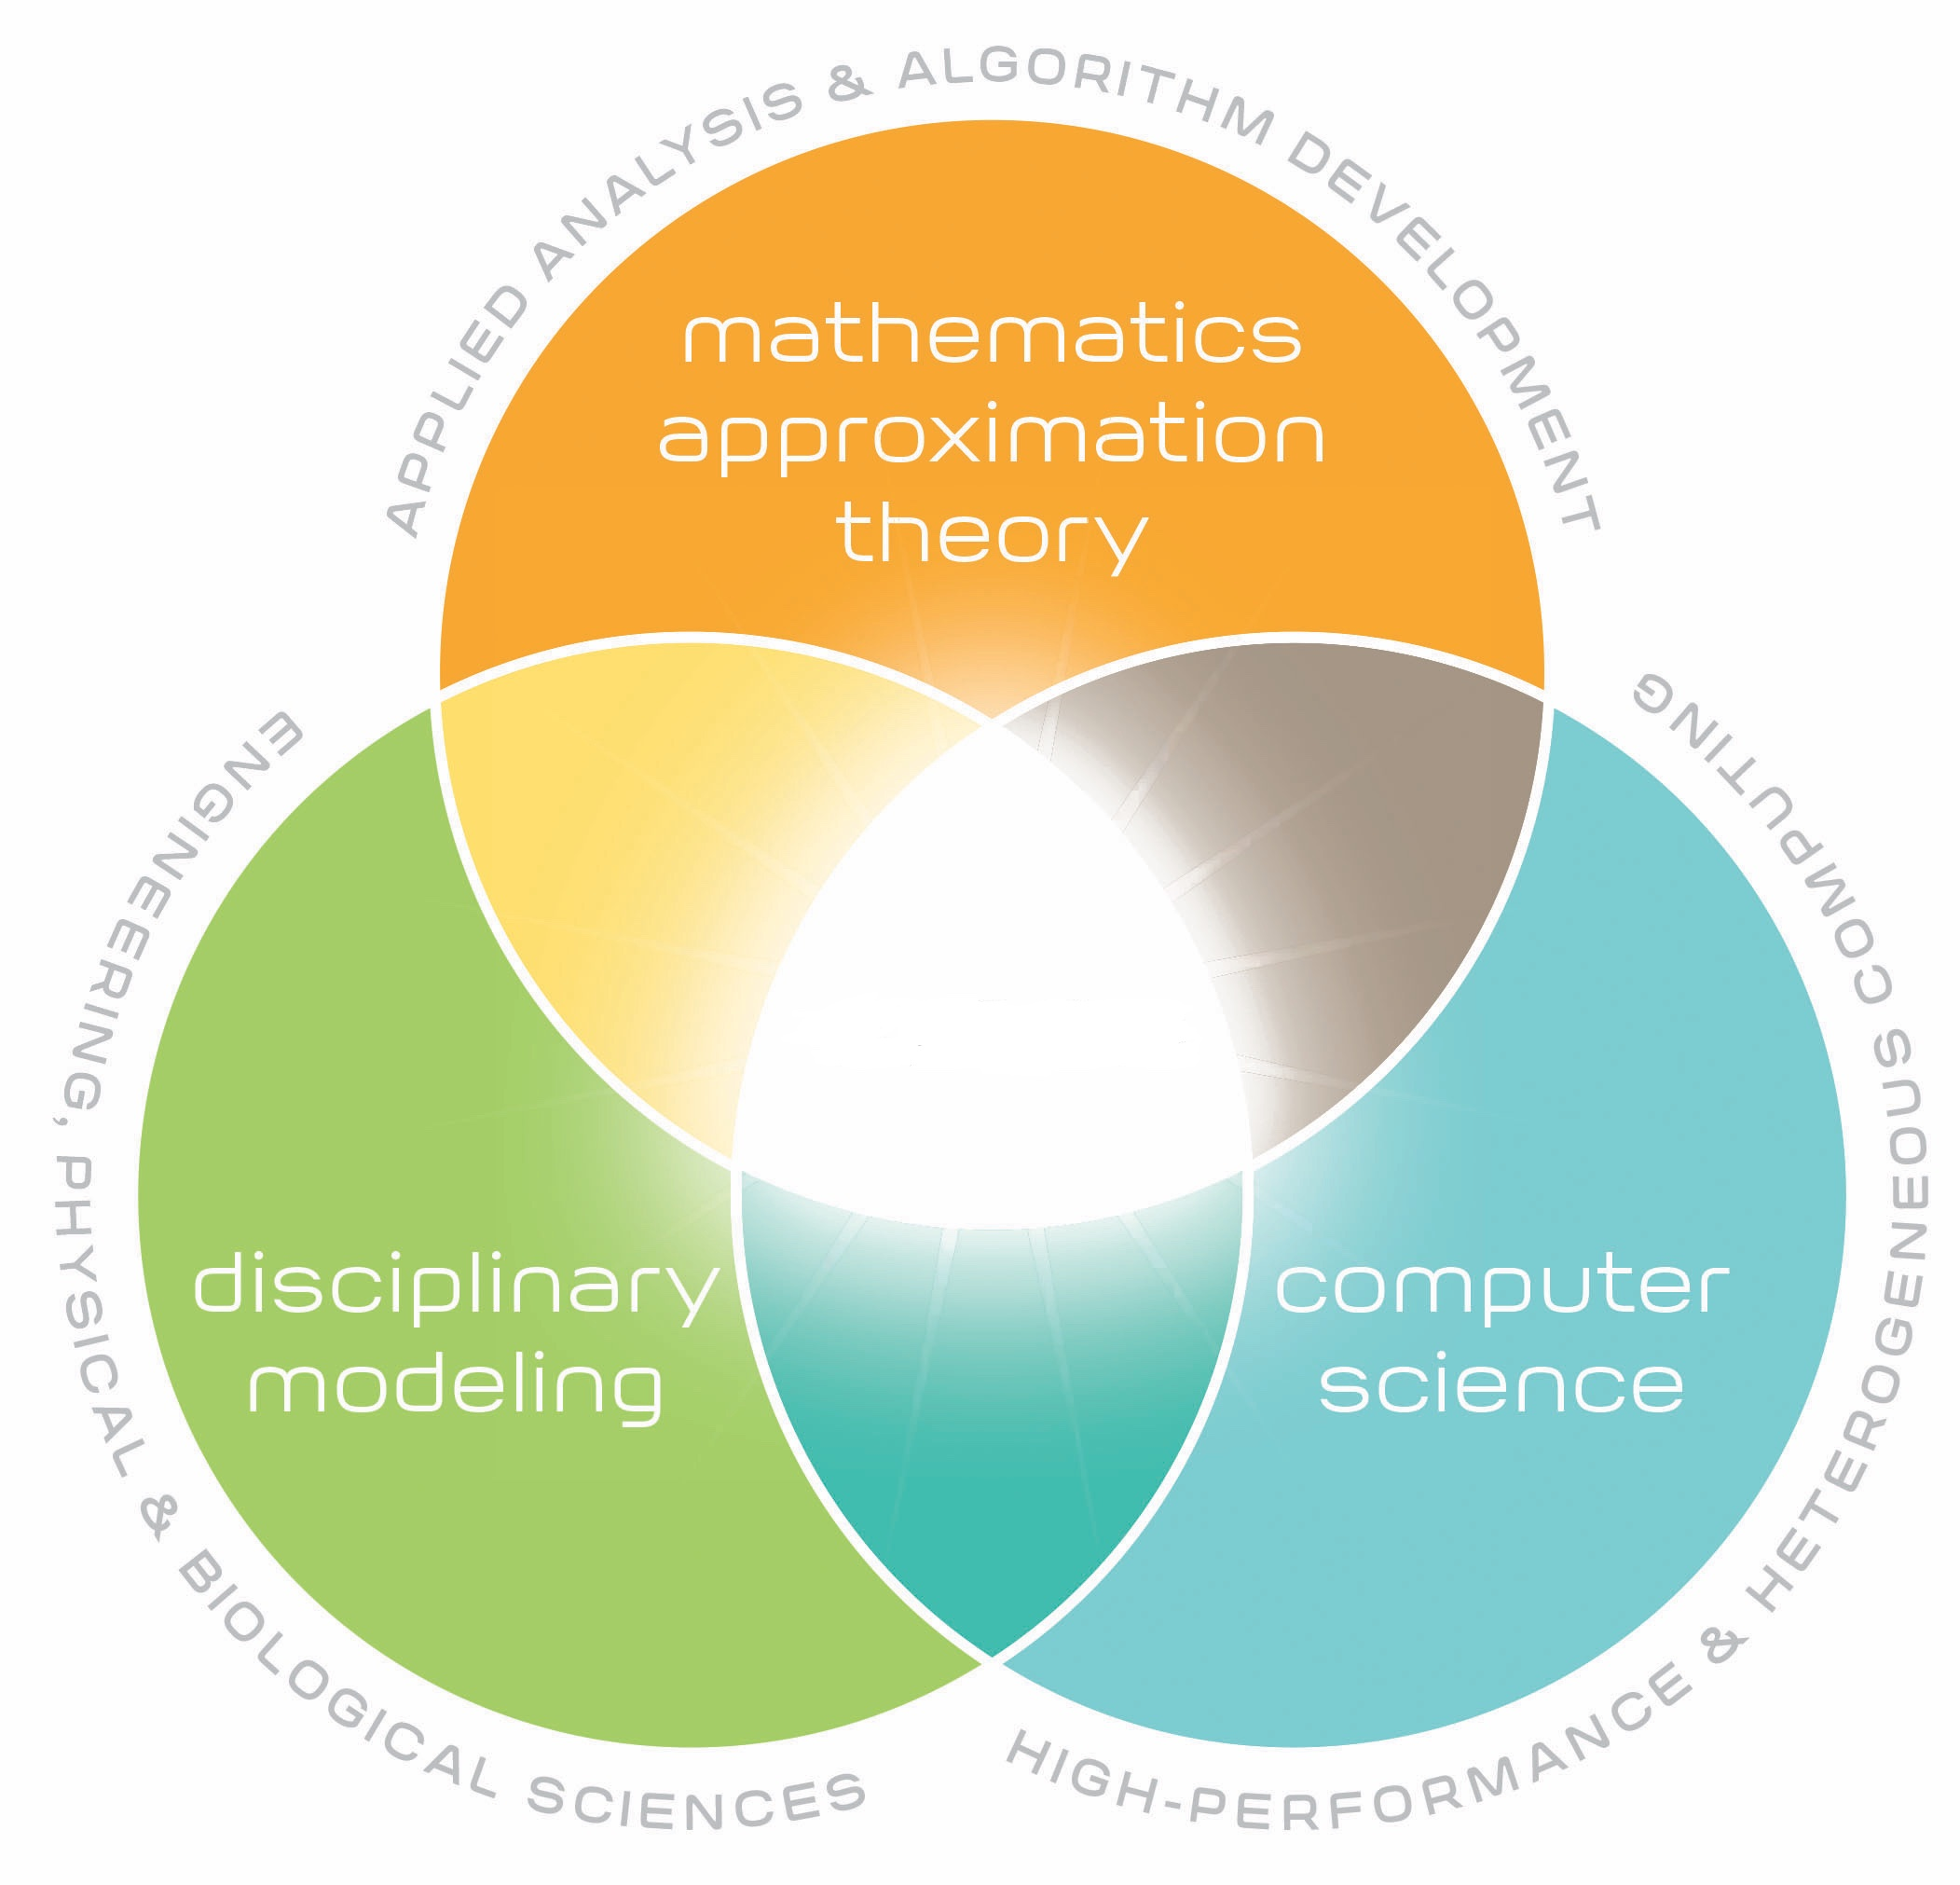
\includegraphics[width=.8\textwidth]{cse.jpg}
				\caption{\href{https://www.uio.no/english/studies/programmes/computational-science-master/why-choose/}{https://www.uio.no}}
			\end{figure}	
			\end{column}
			\begin{column}{.5\textwidth}
			Il s'agit d'une discipline multidisciplinaire, à l'intersection de :
			\begin{itemize}
				\item mathématiques appliquées (analyse numérique, discrétisation des EDP, optimisation);
				\item informatique et développement logiciel;
				\item modélisation physique.
			\end{itemize}
			
			\end{column}
		\end{columns}	
		
	\end{frame}

\begin{frame}{Activités d'enseignement prévues pour le poste}
	L'offre formative ISAE-Supaero prévoit plusieurs cours pour cette discipline.\\
	\vspace{.5cm}
\textbf{Formation ingénieur (FISE)}:
\begin{itemize}
\item 1A : Méthodes numériques EDO et EDP 1D (différences finies, éléments finis).
\item 2A : Équations aux dérivées partielles - Théorie et simulations numériques.
\item 3A : Domaine SXS 
\begin{itemize}
	\item[--] Méthodes numériques pour la mécanique et la fluidodynamique (éléments finis classiques et mixtes, volumes finis);
	\item[--] Calcul Haute performance;
\end{itemize}
\end{itemize}
\vspace{.5cm}
\textbf{Formation Mastère international MAE} :  EDP et calcul scientifique (en anglais).\\
\vspace{.5cm}
\textbf{Formation par Apprentissage (FISA)} : donner aux professionnels les instruments nécessaires pour comprendre les logiciels des simulations.
	
\end{frame}

\begin{frame}{Supervision projets et Création des partenariats}	
Les partenariats industriels sont fondamentales pour les PIR en 2A, les PIE du domaine SXS, et également les stages de fin études.


\begin{columns}
	\begin{column}{.5\textwidth}
	Partenariats industriels : 
	\begin{itemize}
		\item CEA : simulation multiphysique.
		\item CERFACS : CFD et assimilation des données. 
		\item AIRBUS : aéroélasticité et mécanique.
		\item THALES : électromagnétisme, thermoélasticité.
	\end{itemize}
	\end{column}
	\begin{column}{.43\textwidth}
	\begin{figure}
		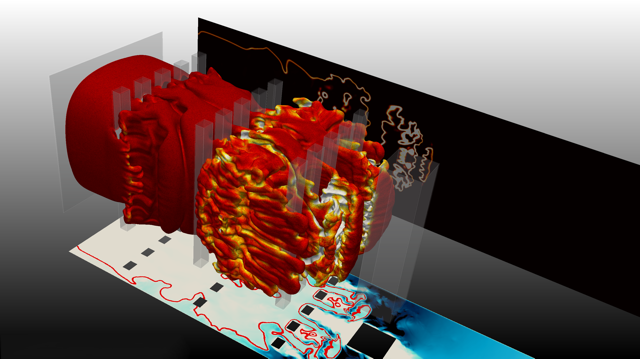
\includegraphics[width=1\textwidth]{image_CERFACS.png}
		\caption{\href{https://cerfacs.fr/logiciels-de-simulation-pour-la-mecanique-des-fluides/}{https://cerfacs.fr}}
	\end{figure}	
	\end{column}
\end{columns}
	
\end{frame}

\section{Projet d'intégration}

\begin{frame}{Analyse numérique et discrétisation des EDP}
	\begin{block}{Discretisation structurée des modeles physiques pour l'ingegnerie}
		Développement des activités de recherche liées à la modélisation et discrétisation structurées des EDP (port-)Hamiltoniennes.
	\end{block}

\begin{columns}		
	\begin{column}{.3\textwidth}
		\includemedia[
		label=vidDam,
		addresource=/home/andrea/Videos/CandidatureISAE/Kirchh_Rod.mp4,
		activate=pageopen,
		width=5cm, height=5cm,
		flashvars={
			source=/home/andrea/Videos/CandidatureISAE/Kirchh_Rod.mp4
			&loop=true
		}
		]{}{VPlayer.swf}
		2D Interconnected plate
	\end{column}
	\begin{column}{.3\textwidth}
		\includemedia[
		label=vidDam,
		addresource=/home/andrea/Videos/CandidatureISAE/vorticity_TG2D.mp4,
		activate=pageopen,
		width=5cm, height=5cm,
		flashvars={
			source=/home/andrea/Videos/CandidatureISAE/vorticity_TG2D.mp4
			&loop=true
		}
		]{}{VPlayer.swf}
		2D Taylor Green
	\end{column}
	\begin{column}{.3\textwidth}
		\includemedia[
		label=vidDam,
		addresource=/home/andrea/Videos/CandidatureISAE/Maxwell_E1_3D.mp4,
		activate=pageopen,
		width=5cm, height=5cm,
		flashvars={
			source=/home/andrea/Videos/CandidatureISAE/Maxwell_E1_3D.mp4
			&loop=true
		}
		]{}{VPlayer.swf}
		3D Maxwell
	\end{column}
\end{columns}	
\mediabutton[
mediacommand=vidNoRod:playPause,
mediacommand=vidRod:playPause
]{\fbox{Play/Pause}}

	
\end{frame}


\begin{frame}{Agenda de recherche}
	
	\begin{block}{Thematique de recherhe}
		\begin{itemize}
			\item Analyse numérique des chemins.
			\item Lien entre géométrie et discrétisation: les éléments finis en calcul extérieur.
			\item Stratégies pour le gain en performance: maillage adaptatif, solveurs et preconditionneurs, parallélisation du code et calcul haute performance. 
			\item Lien vers les applications : mécanique et dynamique des fluides, électromagnétisme, optimisation.
		\end{itemize}

		
	\end{block}
	
	
	\begin{block}{Develloppement logiciel}
		\begin{itemize}
			\item Développement d'un code de calcul pour la multiphysique (SCRIMP).
			\item Création d'un gitlab commun de travail, pour les doctorants, les stagiaires mais également pour le BE et TP des cours lié à la modélisation.
		\end{itemize}	
		
	\end{block}
	
\end{frame}


\begin{frame}{Transversalité au sein du DISC}
	L'intelligence artificielle offre des outils essentielles pour la compression de données issus des chemins de discrétisation.
	
	\begin{figure}[t]
		\begin{subfigure}[t]{0.465\textwidth}
			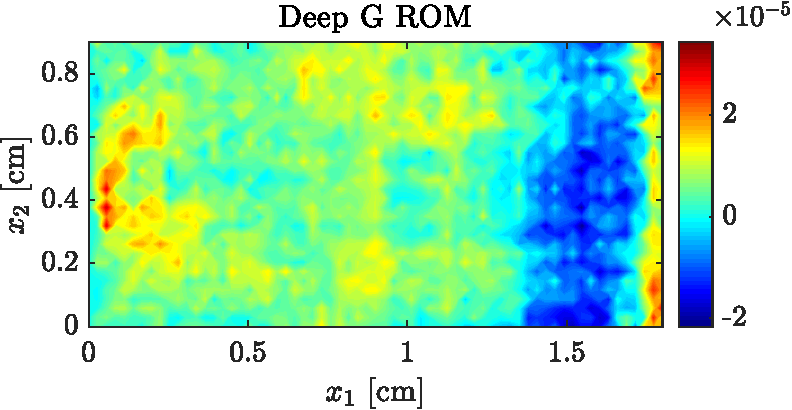
\includegraphics[width=\columnwidth]{DGROM_T_param1.pdf} 
			\caption{Modèle réduit avec réseaux des neurones.}
			\label{fig:DG_ROM}
		\end{subfigure}\hfill
		\begin{subfigure}[t]{0.48\textwidth}
			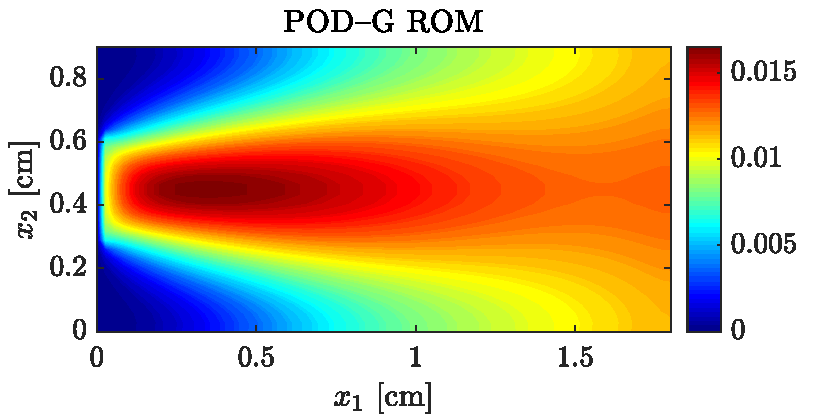
\includegraphics[width=\columnwidth]{GROM_T_param1.pdf}%
			\caption{Modèle réduit avec la méthode linéaire POD.}
			\label{fig:POD_ROM}
		\end{subfigure}
		\caption[]{Erreur des modèles réduits sur le champ de température pour un problème de convection-diffusion-réaction. \\
		Reproduit de \cite{lee2020}.}%
		\label{fig:deepROM}%
	\end{figure}
\end{frame}



\begin{frame}{Transversalité au sein de l'ISAE}


	\begin{block}{Collaborations internes}
		Il est indispensable de collaborer avec différents départements :
		\begin{itemize}
			\item DMSM : mécanique structurelle et optimisation topologique. 
			\item DCAS : pour la réduction des modèles et le contrôle automatique.
			\item DAEP : dynamique des fluides.
		\end{itemize}
	\end{block}

\end{frame}


\begin{frame}{Modules électifs à proposer sur le moyen terme}
Dans le cadre des activités d'enseignement, j'aimerais proposer des cours entre le calcul scientifique et la théorie des systèmes dynamiques.
\begin{itemize}
	\item Modélisation et discrétisation symplectique des structures flexibles complexes.
	\item Éléments de Géométrie différentielle pour la modélisation physique.
\end{itemize}
\end{frame}
	





	
	
\begin{comment}

\end{comment}


\end{document}